\usetikzlibrary{chains, positioning, shapes.geometric, backgrounds, fit}

\definecolor{customYellow}{RGB}{252,226,187}
\definecolor{customBlue}{RGB}{252,224,225}
\definecolor{lightYellow}{RGB}{203,231,207}
\definecolor{lightBlue}{RGB}{243,243,244}

\tikzset{
    box/.style={
        rectangle,
        draw,
        minimum width=1cm,
        minimum height=1cm,
        text centered,
        font=\small\ttfamily
    },
    emb/.style={
        box,
        fill=customYellow
    },
    posi/.style={
        box,
        fill=lightBlue
    },
    segA/.style={
        box,
        fill=lightYellow
    },
    segB/.style={
        box,
        fill=lightYellow
    },
    plus/.style={
        font=\Large,
        text centered
    }
}

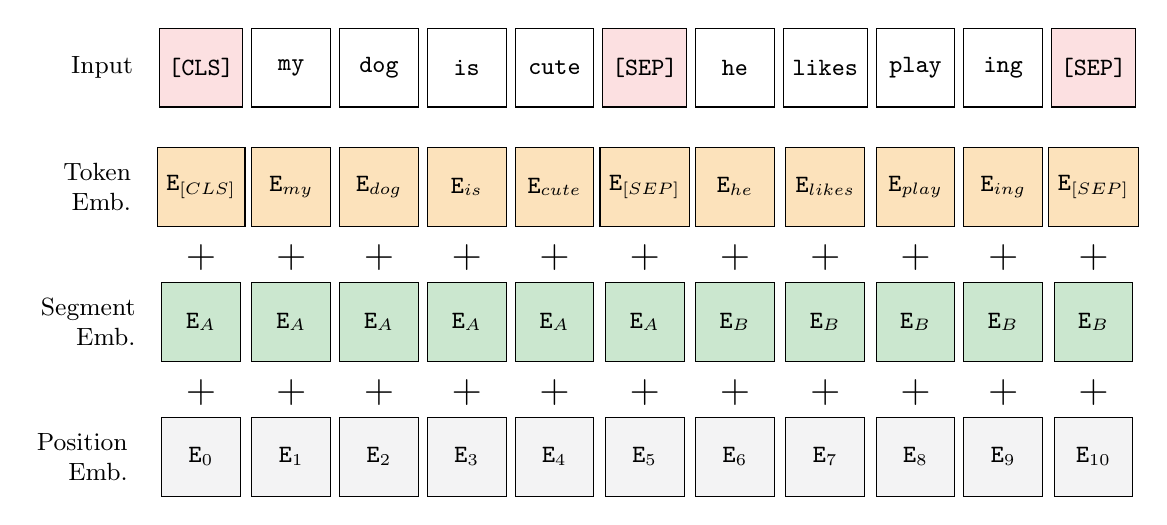
\begin{tikzpicture}[node distance=0.1cm, start chain=1 going right]

% Input boxes
\node [on chain=1, box, fill=customBlue] (in1) {[CLS]};
\node [on chain=1, box] (in2) {my};
\node [on chain=1, box] (in3) {dog};
\node [on chain=1, box] (in4) {is};
\node [on chain=1, box] (in5) {cute};
\node [on chain=1, box, fill=customBlue] (in6) {[SEP]};
\node [on chain=1, box] (in7) {he};
\node [on chain=1, box] (in8) {likes};
\node [on chain=1, box] (in9) {play};
\node [on chain=1, box] (in10) {ing};
\node [on chain=1, box, fill=customBlue] (in11) {[SEP]};

% Token Embeddings
\node [below=0.5cm of in1, emb] (E1) {E$_{[\text{CLS}]}$};
\node [below=0.5cm of in2, emb] (E2) {E$_{my}$};
\node [below=0.5cm of in3, emb] (E3) {E$_{dog}$};
\node [below=0.5cm of in4, emb] (E4) {E$_{is}$};
\node [below=0.5cm of in5, emb] (E5) {E$_{cute}$};
\node [below=0.5cm of in6, emb] (E6) {E$_{[\text{SEP}]}$};
\node [below=0.5cm of in7, emb] (E7) {E$_{he}$};
\node [below=0.5cm of in8, emb] (E8) {E$_{likes}$};
\node [below=0.5cm of in9, emb] (E9) {E$_{play}$};
\node [below=0.5cm of in10, emb] (E10) {E$_{ing}$};
\node [below=0.5cm of in11, emb] (E11) {E$_{[\text{SEP}]}$};

% Plus signs
\node [below=0.1cm of E1, plus] {+};
\node [below=0.1cm of E2, plus] {+};
\node [below=0.1cm of E3, plus] {+};
\node [below=0.1cm of E4, plus] {+};
\node [below=0.1cm of E5, plus] {+};
\node [below=0.1cm of E6, plus] {+};
\node [below=0.1cm of E7, plus] {+};
\node [below=0.1cm of E8, plus] {+};
\node [below=0.1cm of E9, plus] {+};
\node [below=0.1cm of E10, plus] {+};
\node [below=0.1cm of E11, plus] {+};

% Segment Embeddings
\node [below=0.7cm of E1, segA] (SA1) {E$_A$};
\node [below=0.7cm of E2, segA] (SA2) {E$_A$};
\node [below=0.7cm of E3, segA] (SA3) {E$_A$};
\node [below=0.7cm of E4, segA] (SA4) {E$_A$};
\node [below=0.7cm of E5, segA] (SA5) {E$_A$};
\node [below=0.7cm of E6, segA] (SA6) {E$_A$};
\node [below=0.7cm of E7, segB] (SB7) {E$_B$};
\node [below=0.7cm of E8, segB] (SB8) {E$_B$};
\node [below=0.7cm of E9, segB] (SB9) {E$_B$};
\node [below=0.7cm of E10, segB] (SB10) {E$_B$};
\node [below=0.7cm of E11, segB] (SB11) {E$_B$};

% Plus signs
\node [below=0.1cm of SA1, plus] {+};
\node [below=0.1cm of SA2, plus] {+};
\node [below=0.1cm of SA3, plus] {+};
\node [below=0.1cm of SA4, plus] {+};
\node [below=0.1cm of SA5, plus] {+};
\node [below=0.1cm of SA6, plus] {+};
\node [below=0.1cm of SB7, plus] {+};
\node [below=0.1cm of SB8, plus] {+};
\node [below=0.1cm of SB9, plus] {+};
\node [below=0.1cm of SB10, plus] {+};
\node [below=0.1cm of SB11, plus] {+};

% Position Embeddings
\node [below=0.7cm of SA1, posi] (P1) {E$_0$};
\node [below=0.7cm of SA2, posi] (P2) {E$_1$};
\node [below=0.7cm of SA3, posi] (P3) {E$_2$};
\node [below=0.7cm of SA4, posi] (P4) {E$_3$};
\node [below=0.7cm of SA5, posi] (P5) {E$_4$};
\node [below=0.7cm of SA6, posi] (P6) {E$_5$};
\node [below=0.7cm of SB7, posi] (P7) {E$_6$};
\node [below=0.7cm of SB8, posi] (P8) {E$_7$};
\node [below=0.7cm of SB9, posi] (P9) {E$_8$};
\node [below=0.7cm of SB10, posi] (P10) {E$_9$};
\node [below=0.7cm of SB11, posi] (P11) {E$_{10}$};

% Annotations
\node[left=0.2cm of in1, align=right, font=\small]{Input};
\node [left=0.2cm of E1, align=right, font=\small] {Token\\Emb.};
\node [left=0.2cm of SA1, align=right, font=\small] {Segment\\Emb.};
\node [left=0.3cm of P1, align=right, font=\small] {Position\\Emb.};

\end{tikzpicture}
